\subsection{Prospective extension and anchor sensitivity}
A final small extension fixed formaldehyde ($n\pi^*$), ethylene
($\pi\pi^*$) and bright butadiene ($B_u$, $\pi\pi^*$) before their new
predictions. The 50/50 weights, exchange scale 0.9, screened interaction
construction and energy origin were unchanged. All three predictions were
saved before opening their QUEST numerical labels. A bibliographic search
for structural references exposed an approximate formaldehyde vertical value
after its prediction; the extension is therefore described as a prospective
fixed-model test, rather than a strictly blinded experiment. A preparation
amendment replaces a diffuse DFT-TDA seed projection by an explicit native
valence promotion for ethylene and butadiene, followed by the same stationary
KKT and state-fidelity checks. This removes a TDA requirement for these new
state seeds; it does not change the energy model or fit their excitation
energies. The completed formaldehyde prediction retains its original
qualified reference transition.

\begin{center}\begin{tabular}{lrrrr}\toprule
Molecule & Reference & OO-CID & TDA & OO error\\\midrule
Formaldehyde & 3.966 & 4.285 & 4.650 & +0.319\\
Ethylene & 7.897 & 9.079 & 11.430 & +1.182\\
Butadiene & 6.222 & 6.632 & 8.567 & +0.410\\
\bottomrule\end{tabular}
\end{center}
The three-state OO-CID MAE is 0.637 eV, compared with 2.187 eV for the
same-native-orbital TDA response control. OO-CID improves each of these
controls, but ethylene remains 1.182 eV above its reference. The new test
therefore does not sustain a universal 0.5 eV accuracy claim. In particular,
ethylene's minimal valence chart and screened correlation treatment require
further development; the present results do not isolate a single cause.
The two-heavy-atom formaldehyde and ethylene anchors also activate the
specified small frontier fallback because the current heavy-atom-plane
certificate is unavailable. No case is removed or retrospectively refitted.
Fresh public evaluations retain the assigned spin-pure states and pass
restart and no-runtime-DFT/TDA/SCC checks.

\begin{figure}[!htbp]
\centering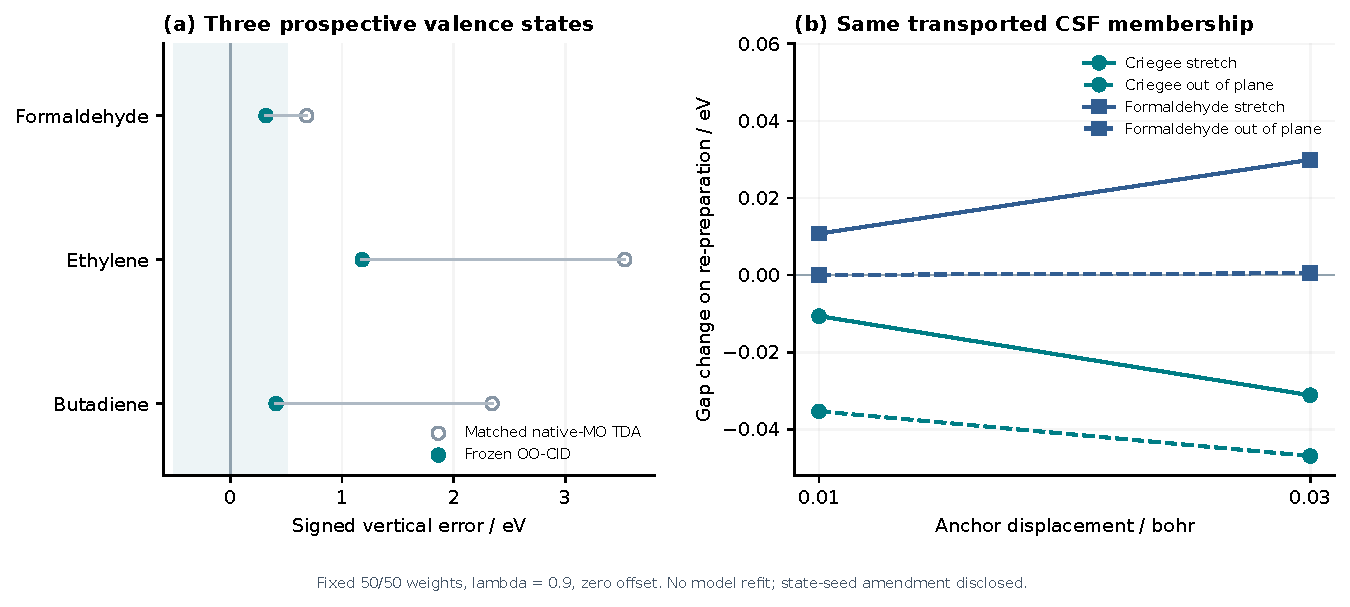
\includegraphics[width=\linewidth]{figures/closing_validation.pdf}
\caption{Final prospective extension and reference-geometry sensitivity.
(a) OO-CID and matched native-orbital TDA signed errors for every new state;
the shaded region is $\pm0.5$ eV. (b) Re-prepared versus original-anchor
excitation gaps evaluated at identical displaced geometries, with the
original CSF membership transported by occupied/virtual orbital overlap.
The model parameters are unchanged. The small extension is separate from
the exposed twenty-state development set.}\label{fig:closingvalidation}
\end{figure}

Anchor tests displace one carbon by 0.01 and 0.03 bohr in an in-plane
stretch or an out-of-plane direction, for the Criegee intermediate and
formaldehyde. Each comparison uses the same physical final geometry,
retains all originally prepared target states and reuses the completed
reference checkpoints. With the original CSF membership transported by
orbital overlap, the largest gap change is 0.047 eV for the Criegee
$\pi\pi^*$ state and 0.030 eV for formaldehyde. These are local controls,
not a bound on arbitrary anchor displacement. Re-selecting the configuration
space at each new anchor is a different operation: loss of the Criegee
reflection certificate reduces its space from 178 to 13 CSFs and changes
the $\pi\pi^*$ gap by 0.263--0.273 eV. A trajectory must retain its frozen
chart; symmetry-dependent space selection must not be silently reapplied
at every displaced geometry. The implemented analytic surface already
retains this membership during nuclear motion.

\subsection{Predecessor structures, frequencies and exact acceleration}
The frozen screened-even predecessor was optimized on the lowest singlet surfaces of
formaldehyde and acetaldehyde using analytic gradients. Full analytic
Hessians then assess the vibrational curvatures. Coupled-cluster internal
coordinates provide a physical structural comparison,\cite{geometries2017}
and selected experimental vibrational fundamentals provide a separately
identified spectroscopic comparison.\cite{formaldehydespectrum1969,acetaldehydespectrum1981}
The model frequencies are unscaled harmonic curvatures, whereas the
experimental numbers are anharmonic level spacings. Modes are assigned
through projections on mass-weighted chemical-coordinate displacement
patterns, rather than matched by frequency order. Inversion splittings and
methyl-torsion level spacings are not used as harmonic curvature references.
Complete coordinates, modes and individual differences are given in the
Supporting Information. These comparisons assess that predecessor energy;
they are not substituted for equilibrium data of the subsequently corrected reference.

A further exact response optimization vectorizes the overlap-residual
completion and avoids scalar derivative-jet allocation for frozen
auxiliary matrix values. A cold two-thread Criegee public-API Hessian takes
397 s, compared with the archived 418 s; energies, gradients and both full
Hessians are bitwise identical between versions. Peak resident memory is
1.19 GB, compared with 1.06 GB. This single-run 4.9\% time reduction is
modest, with other work active on the host, and is not evidence of a
size-scaling improvement or a speed advantage over TDA. The ten algebra,
spin and legacy-contract regressions also pass. No numerical derivative,
Hamiltonian change or fitted correction enters the acceleration.
